\section{Software Security Engineering Solutions}
The need for security-enabled software has introduced several methodologies, standards and tools that can be integrated to the SDLC. This section discusses the different solutions to develop secure software. A great source for developing secure software is OWASP. Although OWASP has many projects, this section will analyze and compare only several of the flagship projects. 

\subsection{The Top Ten}
The OWASP Top Ten is one of the most popular OWASP projects and is recognized by many developers as one of the first steps in producing more secure code. Table \ref{tab:top-10} describes the latest installment of the OWASP Top Ten list. The risks are categorized by the amount of applications tested for a given year (starting in 2017), and the amount of applications with at least one instance of a common weakness enumeration (CWE). This approach provides insight to the OWASP Top Ten team how common each CWE is within the selected applications \cite{owasp_top10_introduction}. 

Although the document exist to bring awareness to the most common vulnerabilities, it has not stopped organizations to use it as a security standard. However, the Top 10 is just the bare minimum of the software security requirements an application should implement. In addition, the risk characteristics of the Top 10 also makes it difficult to thoroughly detect, test or protect against \cite{owasp_top10_as_standard}.

\begin{table}[!h]
    \caption{Top 10 Web Application Security Risks 2021}
    \label{tab:top-10}
    \begin{tabular}{|l|p{30em}|}
        \hline  
        A01:2021 & Broken Access Control \\ 
        \hline
        A02:2021 & Cryptographic Failures \\
        \hline
        A03:2021 & Injection \\
        \hline
        A04:2021 & Insecure Design \\
        \hline
        A05:2021 & Security Misconfiguration \\
        \hline
        A06:2021 & Vulnerable and Outdated Components \\
        \hline
        A07:2021 & Identification and Authentication Failures \\
        \hline
        A08:2021 & Software and Data Integrity Failures \\
        \hline
        A09:2021 & Security Logging and Monitoring Failures \\
        \hline
        A10:2021 & Server-Side Request Forgery (SSRF) \\
        \hline
    \end{tabular}
\end{table}

\subsection{The Application Security Verification Standard}
The Application Security Verification Standard (ASVS) is another flagship project from OWASP that provides an actual standard for application security. The ASVS can be utilized by architects, developers, testers, security professionals, tool vendors, and consumers to define, develop, test and verify secure applications. The most recent version is 4.0, which had a significant change with the adoption of NIST 8000-63-3 Digital Identity Guidelines. The two main objectives of the ASVS are:

\begin{itemize}
    \item to help organizations develop and maintain secure applications
    \item to allow security service vendors, security tools vendors, and consumers to align their requirements and offerings
\end{itemize}

Applications have different security needs and different applications do not need the same level of security. Therefore, the ASVS introduces three security verification levels, each level increasing in complexity. Each level in comprises a list of security requirements that can also be mapped to security-specific features and capabilities that should be built into software as is displayed in Figure \ref{fig:asvs-levels}.
\begin{itemize}
    \item \textbf{Level 1}. Low assurance level, and is completely penetration testable.
    \item \textbf{Level 2}. For applications that contain sensitive data, which requires protection and is the recommended level for most apps
    \item \textbf{Level 3}. For the most critical applications - applications that perform high value transactions, contain sensitive medical data, or any application that requires the highest level of trust.
\end{itemize}
\begin{figure}[!h]
    \centering
    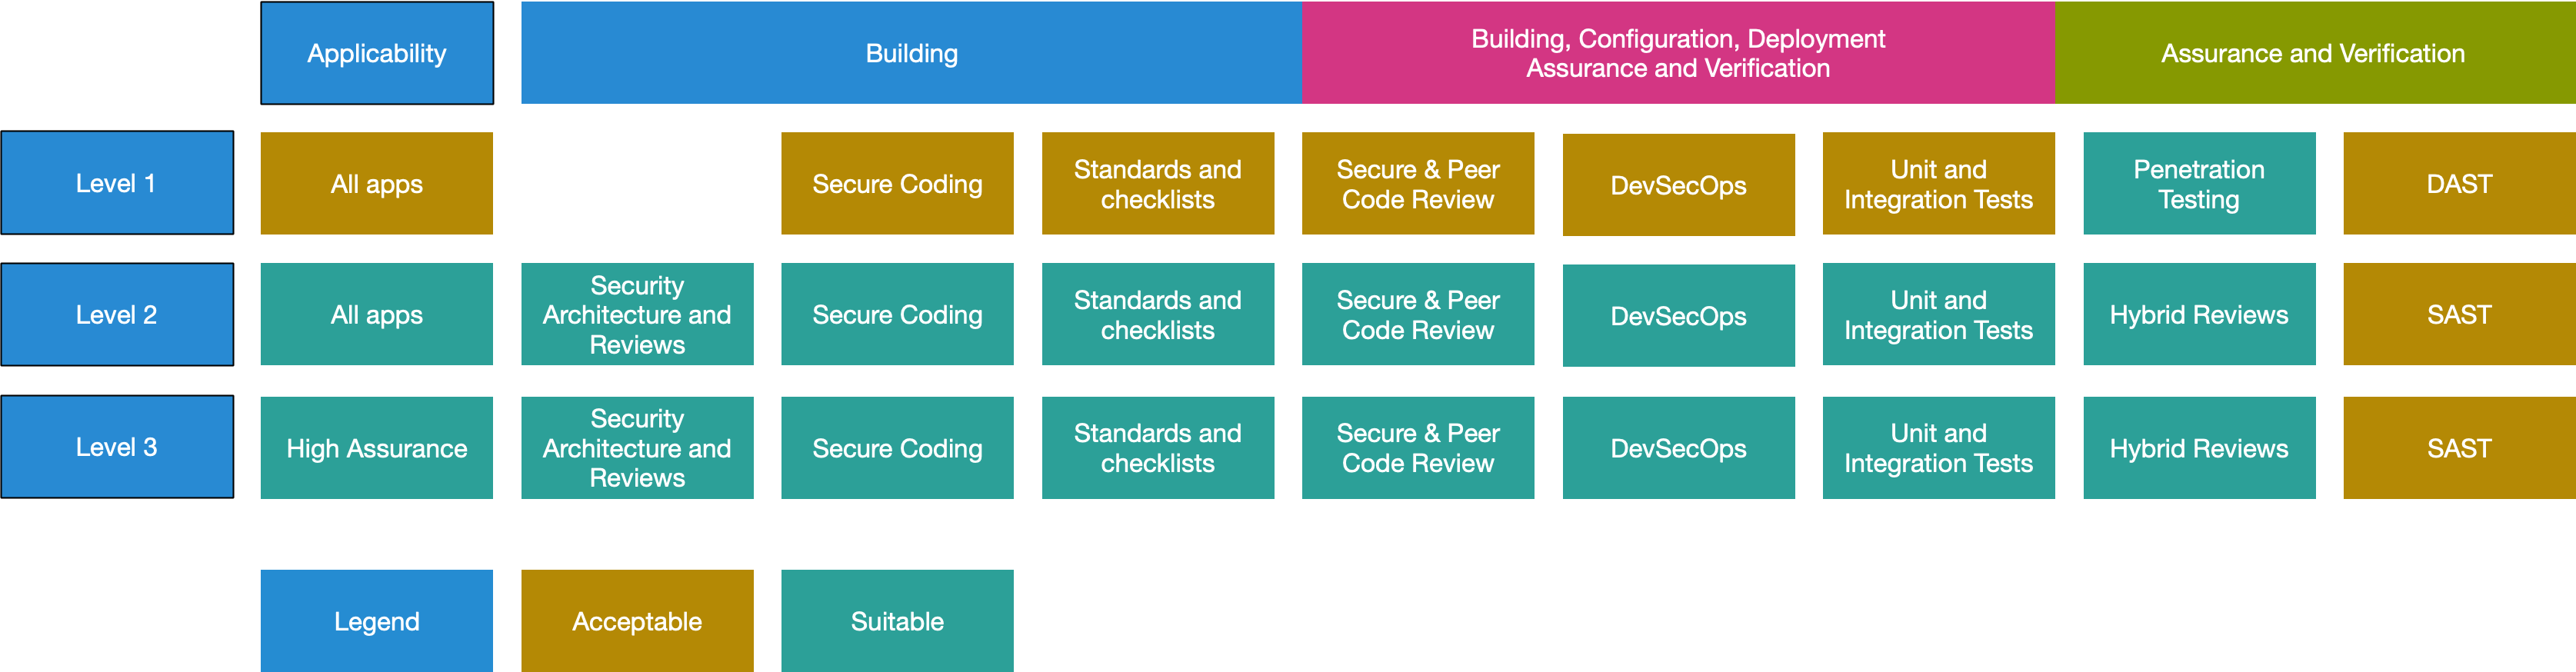
\includegraphics[width=\textwidth]{../../img/chapter_2/owasp-asvs-levels.png}
    \caption{OWASP Application Security Verification Standard 4.0 Levels}
    \label{fig:asvs-levels}
\end{figure}
Unlike Level 2 and Level 3, the security requirements in Level 1 are completely penetration testable. However, in reality it is strongly encouraged to use a broad range of security assurance and verification. Black box testing has proven to be ineffective in identifying critical security issues that led directly to ever more massive breaches \cite{owasp_about}. The usage of security tools like DAST and SAST during the SDLC allows detecting security issues to be found that should not be there in the first place.

\subsubsection{ASVS Level 1}
The bare minimum any application should achieve is that of Level 1, and is useful when the application is not dealing with sensitive data. It sufficiently defends against application security vulnerabilities that are simple to discover by attackers using simple and low level techniques, and are included in the OWASP Top 10 and comparable checklists as well.

\subsubsection{ASVS Level 2}
Most applications today should achieve Level 2, also known as the standard level. Applications achieving Level 2 are generally those that deal with crucial business-to-business transactions or industries where sensitive assets and the integrity is critical to the business.

\subsubsection{ASVS Level 3}

\subsubsection{Security Knowledge Framework}

\subsubsection{Software Assurance Maturity Model}
Whilst the Top 10 functions as an awareness document for security vulnerabilities, and projects like the ASVS and SKF help to identify the security requirements for applications, they do not provide the means to effectively measure the security requirements. The Software Assurance Maturity Model (SAMM) is a tool that can be utilized to help organizations formulate and implement a strategy for software security that is tailored to the specific risks facing the organizations, and can be integrated into the SDLC. An overview of the model can be seen in Table \ref{tab:samm-model}. It describes the four crucial Business Functions together with the three Security Practices that are related to them. Small, medium, large organizations or even individual projects can benefit from the model since SAMM is defined with flexibility in mind. The principles that SAMM was built on are:

\begin{itemize}
    \item An organization's behavior changes slowly over time
    \item No single recipe exist that is applicable to all organizations
    \item Guidance related to security activities must be prescriptive
\end{itemize}

\begin{table}[!h]
    \centering
    \caption{SAMM Model Overview}
    \label{tab:samm-model}
    \begin{tabulary}{1.0\textwidth}{|L|L|L|L|L|}
        \hline
        \textbf{Governance} & \textbf{Implementation} & \textbf{Verification} & \textbf{Operations} \\ 
        \hline
        Strategy and Metrics & Secure Build & Architecture Assessment & Incident Management \\
        \hline
        Policy and Compliance & Secure Deployment & Requirements-driven Testing & Environment Management \\
        \hline
        Education and Guidance & Defect Management & Security Testing & Operational Management \\
        \hline
    \end{tabulary}
\end{table}
